\chapter{Simulación}
En esta sección se presentarán las simulaciones realizadas a través de LTSpiceXVII para medir los parámetros 
característicos del Darlington tanto con carga activa como carga pasiva. Por otro lado, también se desarrollará 
un análisis de Montecarlo para poder observar las sensibilidades del circuito.


\section{Circuito de Polarización}

\subsection{Carga Pasiva}

Primeramente, se realiza la simulación para la polarización del circuito con una carga pasiva de $R_E$ = $900 \Omega$.
\begin{figure}[H]
    \centering
    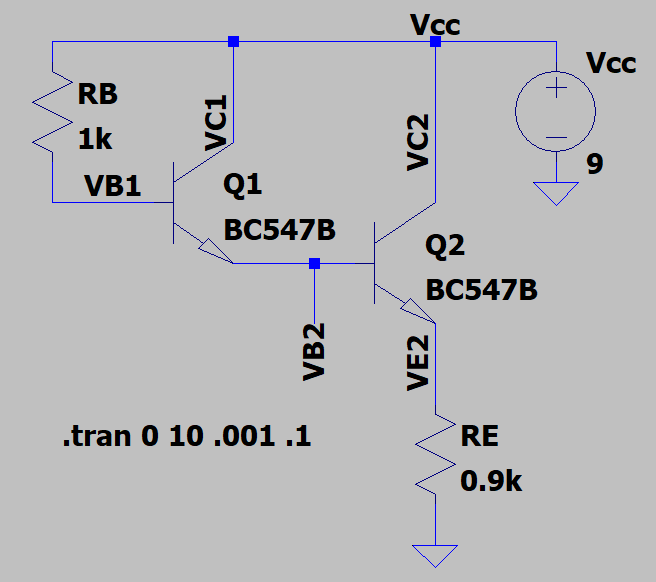
\includegraphics[width=0.5\textwidth]{3_simulacion/fig/circuito_pol_pas.png}
    \label{circuito_pol_pas}
    \caption{Circuito de polarización con carga pasiva}
\end{figure}

Se obtienen los siguientes valores:

\begin{figure}[H]
    \centering
    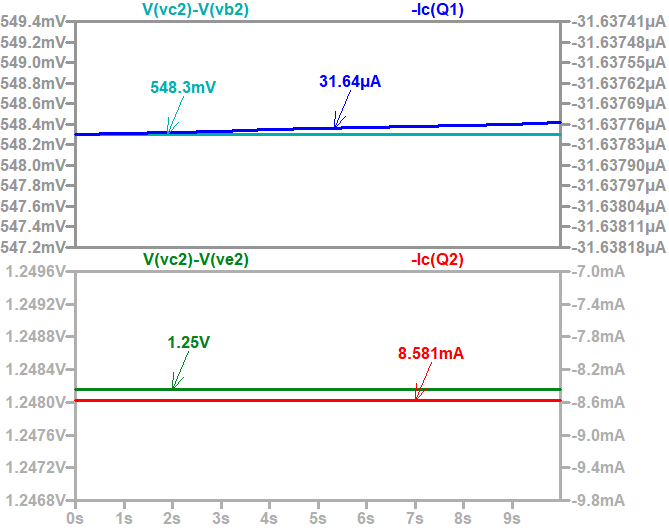
\includegraphics[width=0.75\textwidth]{3_simulacion/fig/pol_pasiva.png}
    \label{mediciones_pol_pas}
    \caption{Mediciones - Circuito de polarización con carga pasiva}
\end{figure}

A continuación se presenta una tabla con las diferencias entre el modelo teórico y simulado:

\begin{table}[H]
    \centering
    \begin{tabular}{|c|c|c|c|}
    \hline
                        & Teórico & Simulado & Error[\%] \\ \hline
    $V_{CE1}[V]$        & $0.6$   & $0.583$  & $2.9$    \\ \hline
    $V_{CE2}[V]$        & $1.2$   & $1.25$   & $4.16$   \\ \hline
    $I_{CQ1}[\mu A]$ & $29.6$  & $31.64$  & $6.89$   \\ \hline  
    $I_{CQ2}[mA]$ & $8.64$  & $8.58$  & $0.69$   \\ \hline
    \end{tabular}
    \end{table}


\subsection{Carga Activa}

Luego, se calcula  para la polarización del circuito con una carga activa implementada con un espejo de corriente.

\begin{figure}[H]
    \centering
    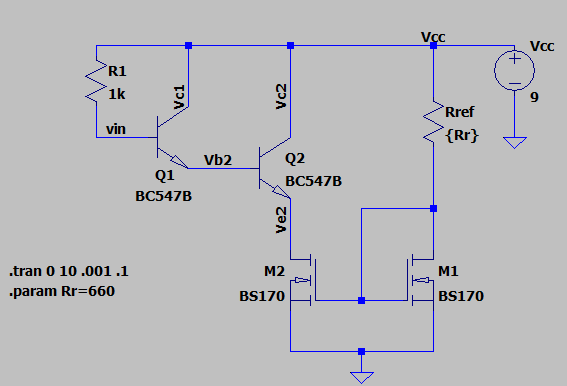
\includegraphics[width=0.5\textwidth]{3_simulacion/fig/circuito_pol_act.png}
    \label{circuito_pol_activa}
    \caption{Circuito de polarización con carga activa}
\end{figure}

Se obtienen los siguientes valores:

\begin{figure}[H]
    \centering
    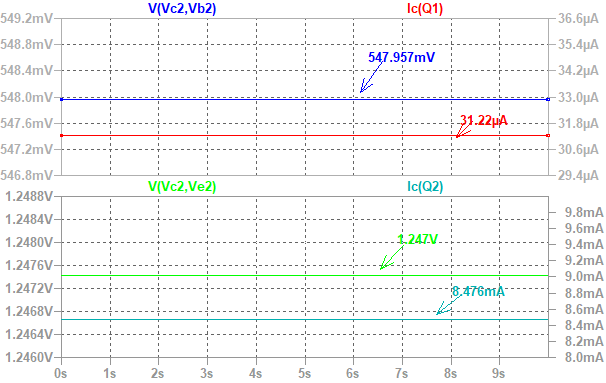
\includegraphics[width=0.75\textwidth]{3_simulacion/fig/pol_activa.png}
    \label{mediciones_pol_activa}
    \caption{Mediciones - Circuito de polarización con carga activa}
\end{figure}
A continuación se presenta una tabla con las diferencias entre el modelo teórico y simulado:

\begin{table}[H]
    \centering
    \begin{tabular}{|c|c|c|c|}
    \hline
                        & Teórico & Simulado & Error[\%] \\ \hline
    $V_{CE1}[V]$        & $0.6$   & $0.547$  & $9.68$    \\ \hline
    $V_{CE2}[V]$        & $1.2$   & $1.247$   & $3.91$   \\ \hline
    $I_{CQ1}[\mu A]$ & $29.6$  & $31.22$  & $5.47$   \\ \hline
    $I_{CQ2}[mA]$ & $8.64$  & $8.48$  & $1.88$   \\ \hline
    \end{tabular}
    \end{table}



\section{Parámetros de Pequeña Señal}
Lorem ipsum
\section{Circuito Incremental}
Lorem ipsum
\subsection{Ganancia de Tensión}
\subsection{Ganancia de Corriente}
Lorem ipsum
\subsection{Impedancias de Entrada y Salida}
Para la impedancia de entrada se realiza la siguiente simulación:
\begin{figure}[H]
    \centering
    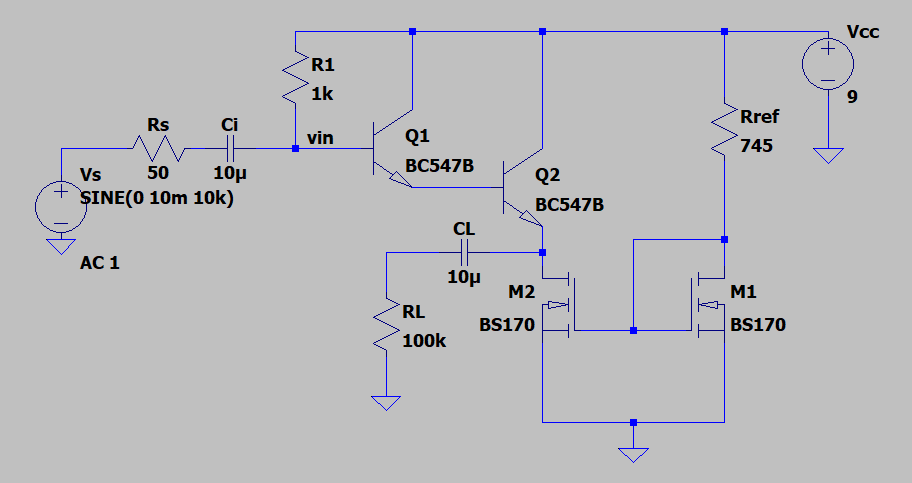
\includegraphics[width=0.75\textwidth]{3_simulacion/fig/circuito_rin.png}
    \label{mediciones_pol_activa}
    \caption{Mediciones - Circuito de polarización con carga activa}
\end{figure}
Obteniéndose los siguientes valores para la impedancia de entrada:
\begin{figure}[H]
    \centering
    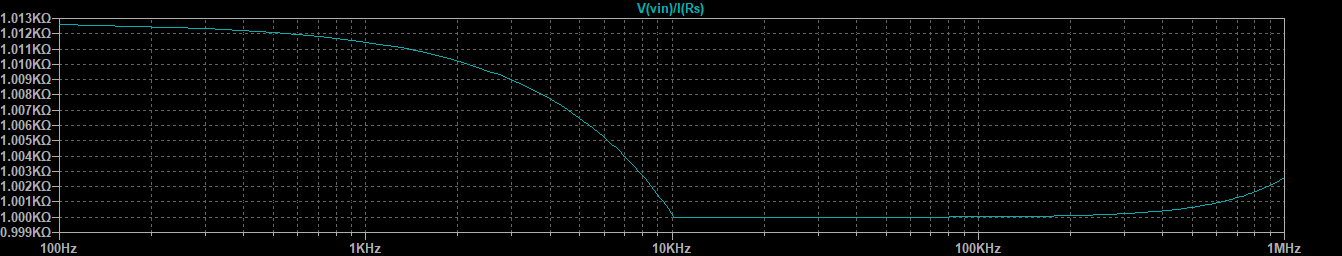
\includegraphics[width=0.75\textwidth]{3_simulacion/fig/rin.png}
    \label{mediciones_pol_activa}
    \caption{Mediciones - Circuito de polarización con carga activa}
\end{figure}

Para la impedancia de salida se realiza la siguiente simulación:
\begin{figure}[H]
    \centering
    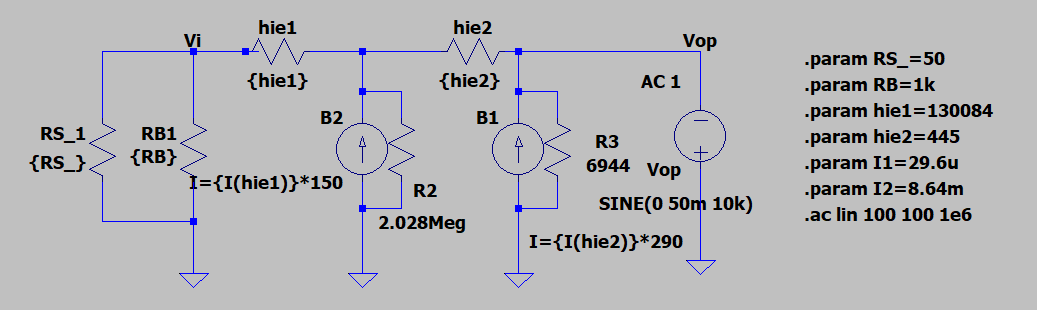
\includegraphics[width=0.75\textwidth]{3_simulacion/fig/circuito_ro.png}
    \label{mediciones_pol_activa}
    \caption{Mediciones - Circuito para medir impedancia de salida}
\end{figure}

Lorem ipsum
\subsection{Respuesta en Frecuencia}
Lorem ipsum